\documentclass{article}

% if you need to pass options to natbib, use, e.g.:
% \PassOptionsToPackage{numbers, compress}{natbib}
% before loading nips_2016
%
% to avoid loading the natbib package, add option nonatbib:
% \usepackage[nonatbib]{nips_2016}

%\usepackage{nips_2016}

% to compile a camera-ready version, add the [final] option, e.g.:
 \usepackage[final]{nips_2016}

\usepackage[utf8]{inputenc} % allow utf-8 input
\usepackage[T1]{fontenc}    % use 8-bit T1 fonts
\usepackage{hyperref}       % hyperlinks
\usepackage{url}            % simple URL typesetting
\usepackage{booktabs}       % professional-quality tables
\usepackage{amsfonts}       % blackboard math symbols
\usepackage{nicefrac}       % compact symbols for 1/2, etc.
\usepackage{microtype}      % microtypography
\usepackage{graphicx}

\title{Category Classification With Animal Image Data}

% The \author macro works with any number of authors. There are two
% commands used to separate the names and addresses of multiple
% authors: \And and \AND.
%
% Using \And between authors leaves it to LaTeX to determine where to
% break the lines. Using \AND forces a line break at that point. So,
% if LaTeX puts 3 of 4 authors names on the first line, and the last
% on the second line, try using \AND instead of \And before the third
% author name.

\author{
 Chudan Liu\\
 Harvey Mudd College\\
 Claremont, CA 91711 \\
 \texttt{iliu@g.hmc.edu} \\
 %% examples of more authors
  \And
  Xinyu Yang \\
  Harvey Mudd College \\
  Claremont, CA 91711 \\
  \texttt{xiyang@g.hmc.edu} \\
 %% \And
 %% Coauthor \\
 %% Affiliation \\
 %% Address \\
 %% \texttt{email} \\
}
\begin{document}
% \nipsfinalcopy is no longer used

\maketitle

\begin{abstract}
\end{abstract}

\section{Introduction}
\paragraph{}
	In this paper we are dealing with image classification problem, which is the job of assigning an input image one label from a fixed set of categories. This is one of the core problems in Computer Vision that, despite its simplicity, has a large variety of practical applications. Moreover many other seemingly distinct Computer Vision tasks (such as object detection, segmentation) can be reduced to image classification.
	
The task in Image Classification is to predict a single label (or a distribution over labels as shown here to indicate our confidence) for a given image. Images are 3-dimensional arrays of integers from 0 to 255, of size Width x Height x 3. The 3 represents the three color channels Red, Green, Blue. For the sake of our future implementation, we transfer the RGB into grayscale image. 
\\
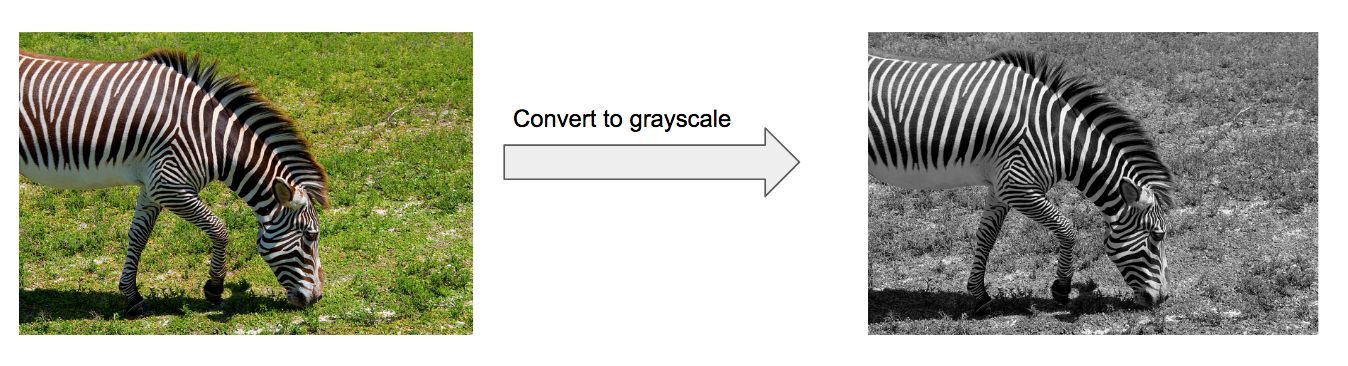
\includegraphics[scale=0.57]{1.png}

\paragraph{}
For this project, we selected the Common Object in Context (COCO) dataset \url{http://mscoco.org/dataset}, a popular image recognition, segmentation, and captioning dataset to perform image classification. We chose this dataset because it has over 80,000 images with multiple objects and clear labels. Before discussing the classifier used in this project, we would first introduce our data construction. In this project, we chose the logistic regression model and a multi-layer perceptron neural network model to classify our data and make the prediction. 

\section{Data Processing}
\label{gen_inst}
We used some open-source software libraries to facilitate the implementation, including sklearn \url{http://scikit-learn.org/stable/}, opencv (Open Source Computer Vision Library) \url{opencv.org/}, numpy \url{http://www.numpy.org/}, and matplolib \url{https://matplotlib.org}. For algorithm, we used the logistic regression model, support vector machine(svm) and neural network module in sklearn to train and test our data with different algorithms. To analyze the performance of our prediction, we plot the confusion matrix using the matrix class in sklearn.
\subsection{Introduction to the COCO dataset}

\paragraph{}
COCO is a popular image recognition, segmentation, and captioning dataset with more than 30,000 images, 2 million instances, and 80 object categories. In this project, we used the 2014 dataset for detection challenge with object instance annotations provided as our primary dataset. For this dataset, there are total 82,782 images of over 90 different categories. 
\paragraph{}
The dataset are in json format, providing comprehensive information. Each annotation instance contains a series of fields, including the category id and segmentation mask of the object, which provides information including the information of the dataset, the categories and supercategories each image belong to and information about segmentation, etc.
\paragraph{}
In this project, we looked into each annotation instance and created our final dataset using images with supercategory ‘animal.’ For this supercategory in particular, there are ten categories shown as below:

\begin{verbatim}
{'id': 16, 'name': 'bird', 'supercategory': 'animal'},
{'id': 17, 'name': 'cat', 'supercategory': 'animal'},
{'id': 18, 'name': 'dog', 'supercategory': 'animal'},
{'id': 19, 'name': 'horse', 'supercategory': 'animal'},
{'id': 20, 'name': 'sheep', 'supercategory': 'animal'},
{'id': 21, 'name': 'cow', 'supercategory': 'animal'},
{'id': 22, 'name': 'elephant', 'supercategory': 'animal'},
{'id': 23, 'name': 'bear', 'supercategory': 'animal'},
{'id': 24, 'name': 'zebra', 'supercategory': 'animal'},
{'id': 25, 'name': 'giraffe', 'supercategory': 'animal'}
\end{verbatim}

\subsection{Assigning training and testing data sets}

\paragraph{}
Considering the enormous size of the whole dataset, we found it infeasible to train the whole dataset based on the current device we have. Instead, we selected one supercategory 'animal', which contains ten different categories or species shown above. We first extracted all images labeled with $category\_ id$ that belongs to the supercategory 'animals,' which consist of over 19,000 images. After we obtained all animal images, we randomly sample 5,000 images as our final full dimension dataset. 
\paragraph{}
We divided the dataset by assigning $3 \slash 4$ of the data, 3750 images, to our training set and the rest of $1\slash 4$, 1250 images, to the testing set. When we sampled the dataset, we shuffled the dataset so that images of most categories under this supercategory are included in the dataset.

\subsection{Dimension analysis}

\section{Learning Algorithms}
\paragraph{}
In our project, we used two algorithms to classify the data: multinomial Logistic Regression and muli-layer perceptron neural network(MLP). Below are details about the algorithm we used in this project. 
\subsection{Multinomial Logistic Regression}
\paragraph{}
Multinomial Logistic Regression is the first learning algorithm we used. Given a set of independent categorical variables, which are the pixels of animal images from our dataset in this case, we trained a logistic regression model to predict the probabilities of the different possible animals of the independent  categorical variables. 
\paragraph{}
As most other statistical classification models, the foundation of the multinomial logistic regression model is to construct a linear predictor function that computes a score from a set of regression coefficients  that indicate the relative effect of variables on the $y$. In particular, \[
Score(k, X_i) = \beta_k \cdot X_i,
\]
where $k$ indicates the $k^{th}$ outcome of , $X_i$ is the vector of explanatory variables, which are all the pixels of an image describing observation i, $\beta_k$ is a vector of  regression coefficients corresponding to outcome k.

\paragraph{}
In terms of actual implementation, we added a regulation parameter $ \ reg=0.2\ $ to prevent the case of overfitting. To analyze the model's performance, we computed the accuracy and generated confusion matrix based on the training set and the test set.

\subsection{Multi-layer Perceptron(MLP) Classifier}
\paragraph{}
Multi-layer Perceptron (MLP) \url{http://scikit-learn.org/stable/modules/neural_networks_supervised.html} is a supervised learning algorithm with multiple hidden layers. It inputs a set of $m$ features \[
X = x_1, x_2, ... , x_m\]
and an output function $f(X)$, learns a non-linear function approximator for either classification or regression. In our implementation, we used the class MLP Classifier in sklearn library. We set the solver as  'adam,' a stochastic gradient-based optimizer proposed by Kingma, Diederik, and Jimmy Ba \url{https://arxiv.org/abs/1412.6980}. We originally set the hidden layer size as (100,100,100), which included three hidden layers, each has size 100, and we also added L2 penalty (regularization term) parameter.

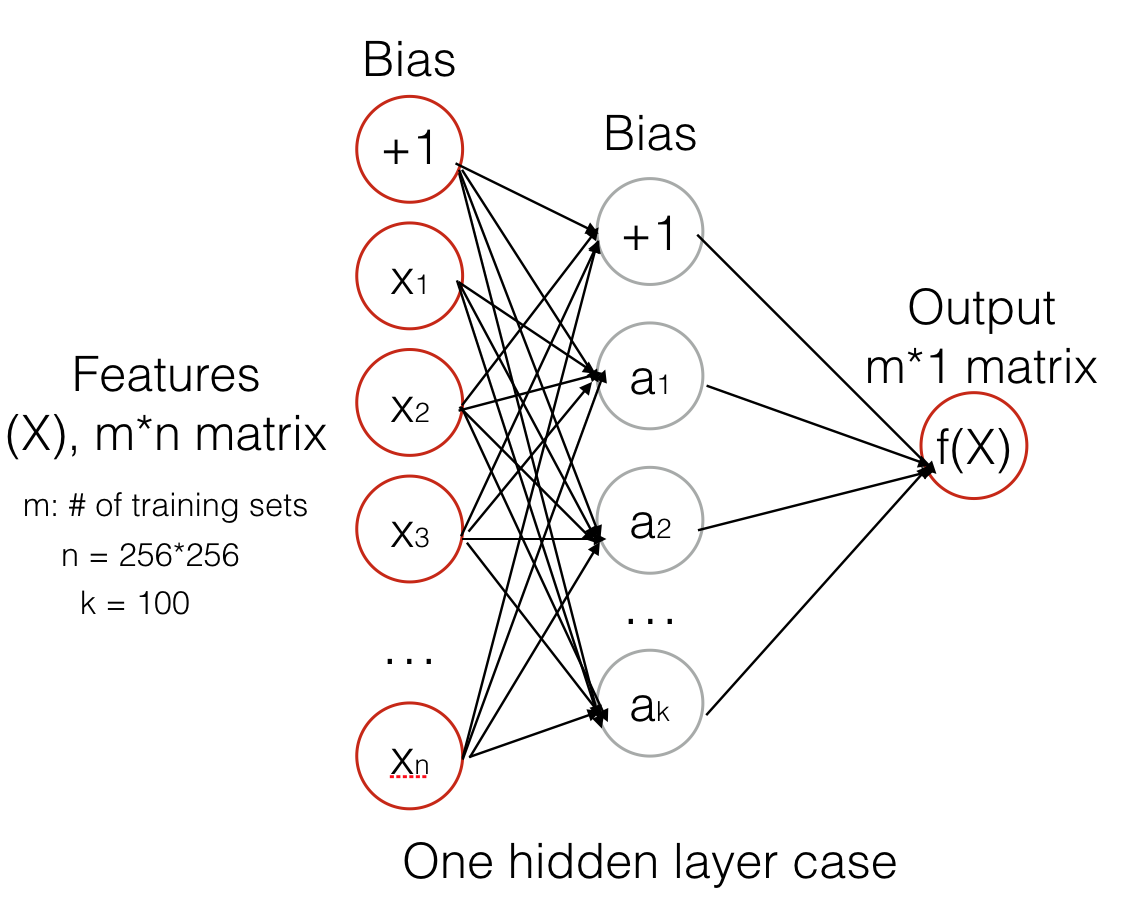
\includegraphics[scale=0.5]{2.png}\\

\paragraph{}
As someone may ask, given the logistic regression model, why do we need multi-layer perceptrons to classify dataset. Comparing with logistic regression, the advantage of multi-layer perceptrons is the capability to learn non-linear models. However, different random weight initializations can have different test accuracy because MLP with hidden layers have a non-convex loss function where there exists more than one local minimum. 

\section{Performance and Analysis}
\subsection{Evaluate Performance: Confusion Matrix}
\subsection{Performance of Multinomial Logistic Regression} Testing Accuracy analysis: 

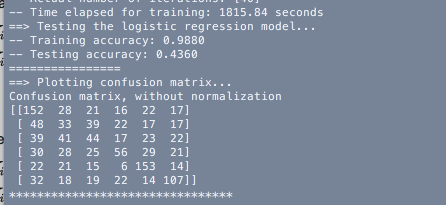
\includegraphics[scale=0.7]{3.png}
\\
Confusion matrix analysis: 
\\
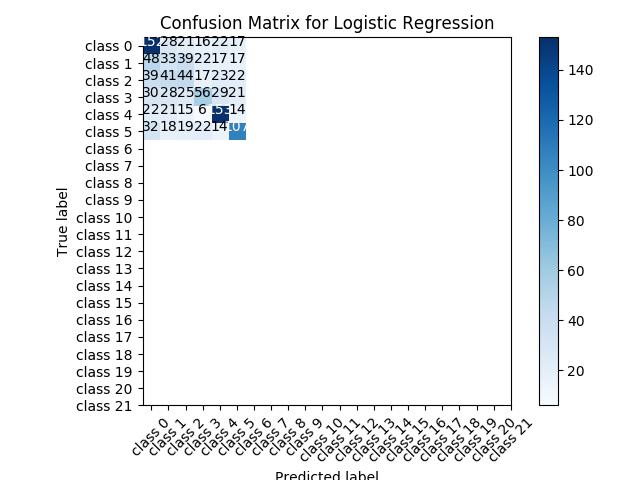
\includegraphics[scale=0.4]{logreg_cm.png}

\subsection{Performance of Multi-layer Perceptrons}

Testing Accuracy analysis: 

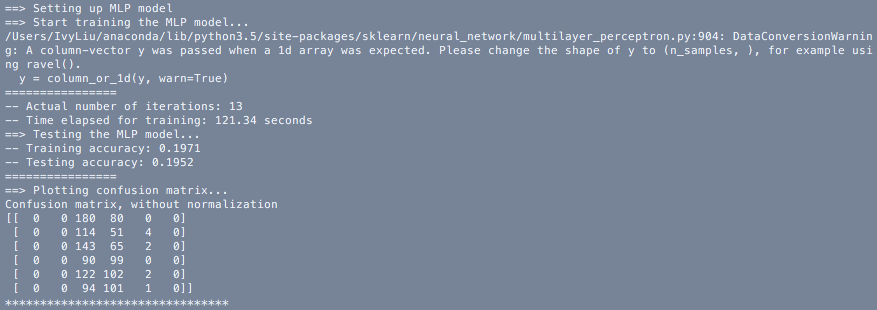
\includegraphics[scale=0.4]{4.png}
\\
Confusion matrix analysis: 
\\
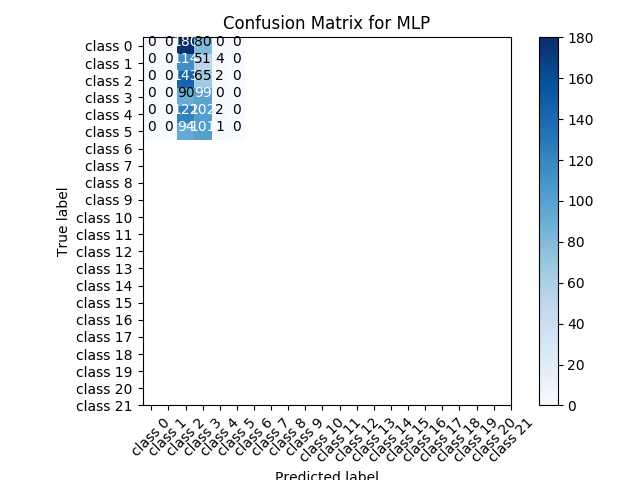
\includegraphics[scale=0.4]{MLP_cm.png}

\subsection{Performance of Linear SVM}

Testing Accuracy analysis: 

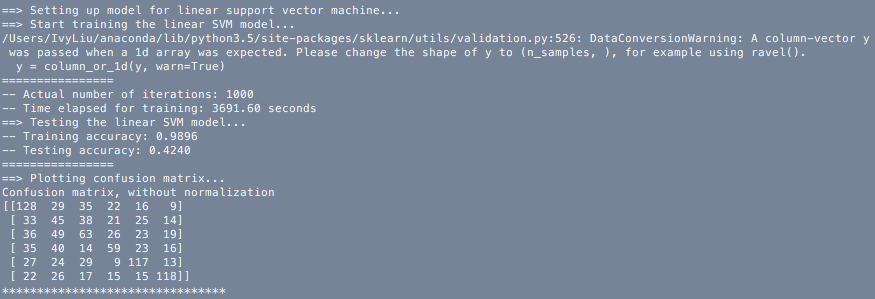
\includegraphics[scale=0.4]{5.png}
\\
Confusion matrix analysis: 
\\
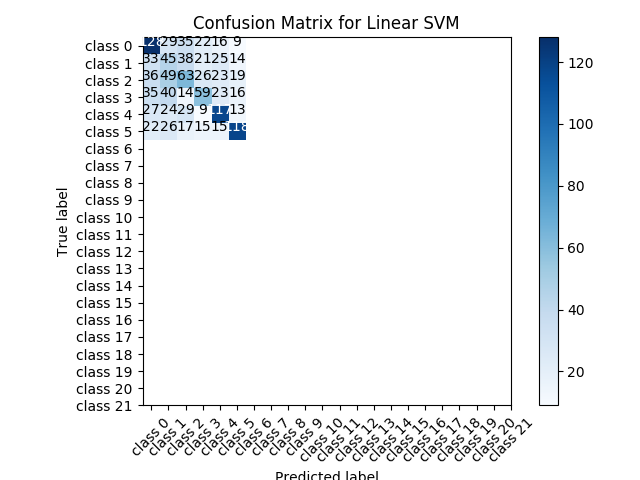
\includegraphics[scale=0.4]{linsvm_cm.png}

\section{Conclusion}

\section*{References}

References follow the acknowledgments. Use unnumbered first-level
heading for the references. Any choice of citation style is acceptable
as long as you are consistent. It is permissible to reduce the font
size to \verb+small+ (9 point) when listing the references. {\bf
  Remember that you can use a ninth page as long as it contains
  \emph{only} cited references.}
\medskip

\small

[1] Alexander, J.A.\ \& Mozer, M.C.\ (1995) Template-based algorithms
for connectionist rule extraction. In G.\ Tesauro, D.S.\ Touretzky and
T.K.\ Leen (eds.), {\it Advances in Neural Information Processing
  Systems 7}, pp.\ 609--616. Cambridge, MA: MIT Press.

[2] Bower, J.M.\ \& Beeman, D.\ (1995) {\it The Book of GENESIS:
  Exploring Realistic Neural Models with the GEneral NEural SImulation
  System.}  New York: TELOS/Springer--Verlag.

[3] Hasselmo, M.E., Schnell, E.\ \& Barkai, E.\ (1995) Dynamics of
learning and recall at excitatory recurrent synapses and cholinergic
modulation in rat hippocampal region CA3. {\it Journal of
  Neuroscience} {\bf 15}(7):5249-5262.

\end{document}